\documentclass[border=4pt]{standalone}
\usepackage{tikz}
\usepackage{amsmath,amssymb}
\usepackage{mathptmx}
\usetikzlibrary{arrows.meta,positioning,calc,shapes.geometric,decorations.pathreplacing,shadows,fadings,patterns}
\definecolor{cblue}{HTML}{1F4E9C}
\definecolor{cgold}{HTML}{D08C00}
\definecolor{cred}{HTML}{B5172E}
\definecolor{cgreen}{HTML}{1B7A3A}
\definecolor{cgrey}{HTML}{555555}
\definecolor{cpurple}{HTML}{5B2A86}
% oblique 3D cuboid: \cuboid{x}{y}{z}{dx}{dy}{dz}{colour}
\newcommand{\cuboid}[7]{%
  \fill[#7!55!white,draw=#7!60!black,line width=0.4pt] (#1,#2,#3+#6) -- ++(#4,0,0) -- ++(0,#5,0) -- ++(-#4,0,0) -- cycle;
  \fill[#7!80!black,draw=#7!60!black,line width=0.4pt] (#1+#4,#2,#3) -- ++(0,#5,0) -- ++(0,0,#6) -- ++(0,-#5,0) -- cycle;
  \fill[#7,draw=#7!60!black,line width=0.4pt] (#1,#2,#3) -- ++(#4,0,0) -- ++(0,0,#6) -- ++(-#4,0,0) -- cycle;}

\begin{document}
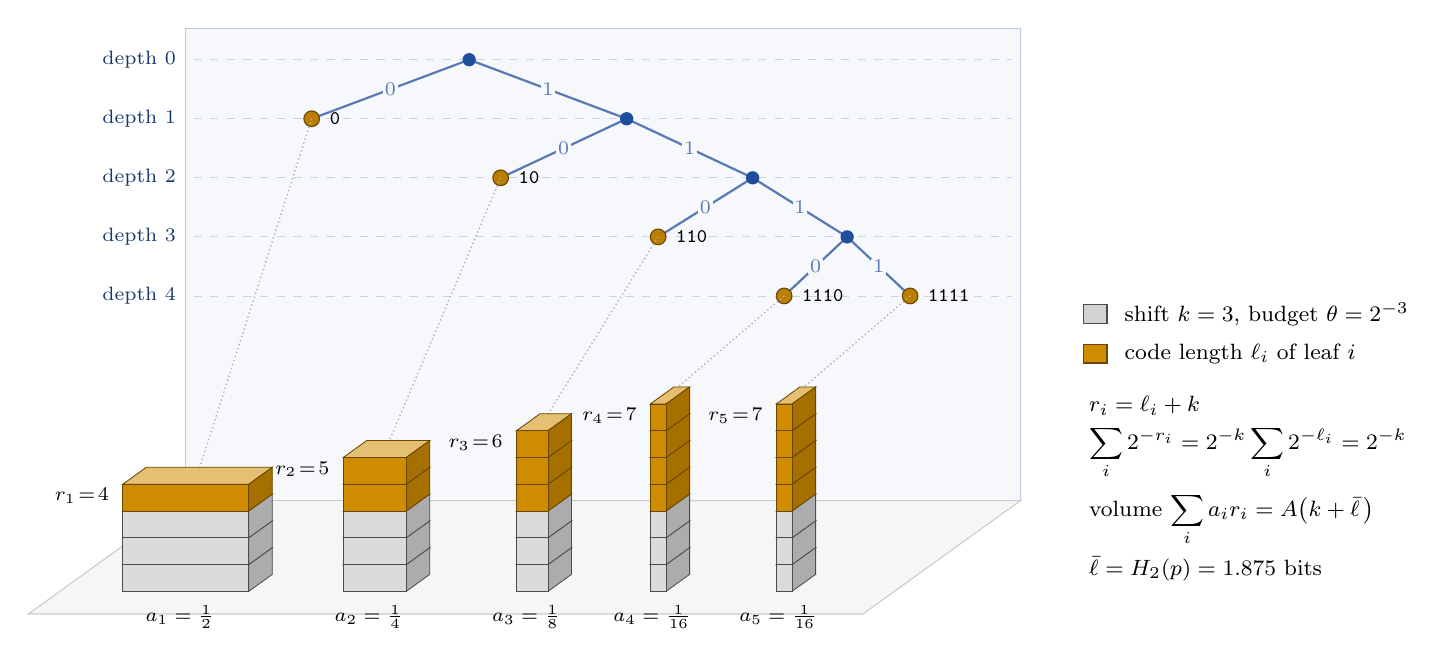
\begin{tikzpicture}[x={(1cm,0cm)},y={(0.5cm,0.36cm)},z={(0cm,1cm)},
  nd/.style={circle,fill=cblue,inner sep=1.7pt},
  lf/.style={circle,fill=cgold!90!black,draw=cgold!50!black,inner sep=2pt}]
\def\h{0.34}
\def\wy{3.2}
% back wall carrying the code tree
\fill[cblue!4,draw=cblue!30] (-0.6,\wy,0) -- (10.0,\wy,0) -- (10.0,\wy,6.0) -- (-0.6,\wy,6.0) -- cycle;
\foreach \d in {0,...,4}{
  \pgfmathsetmacro\zz{5.6-0.75*\d}
  \draw[cblue!25,dashed,line width=0.3pt] (-0.5,\wy,\zz) -- (9.9,\wy,\zz);
  \node[font=\scriptsize,cblue!70!black,anchor=east] at (-0.6,\wy,\zz) {depth \d};}
% floor
\fill[gray!7,draw=gray!40] (-0.6,-0.8,0) -- (10.0,-0.8,0) -- (10.0,\wy,0) -- (-0.6,\wy,0) -- cycle;
% tree coordinates on the wall
\coordinate (R)  at (3.0,\wy,5.6);
\coordinate (N1) at (5.0,\wy,4.85);
\coordinate (N2) at (6.6,\wy,4.1);
\coordinate (N3) at (7.8,\wy,3.35);
\coordinate (L1) at (1.0,\wy,4.85);
\coordinate (L2) at (3.4,\wy,4.1);
\coordinate (L3) at (5.4,\wy,3.35);
\coordinate (L4) at (7.0,\wy,2.6);
\coordinate (L5) at (8.6,\wy,2.6);
\foreach \a/\b/\bit in {R/L1/0,R/N1/1,N1/L2/0,N1/N2/1,N2/L3/0,N2/N3/1,N3/L4/0,N3/L5/1}
  \draw[cblue!75,line width=0.8pt] (\a) -- (\b) node[midway,font=\scriptsize,fill=cblue!4,inner sep=0.6pt] {\bit};
\foreach \c in {R,N1,N2,N3} \node[nd] at (\c) {};
\foreach \c/\cw in {L1/0,L2/10,L3/110,L4/1110,L5/1111}{
  \node[lf] at (\c) {};
  \node[font=\scriptsize,anchor=west,xshift=3pt] at (\c) {\texttt{\cw}};}
% columns: base width proportional to a_i; three grey shift blocks and l_i gold code blocks
\foreach \x/\w/\l/\name/\code in {1.0/1.6/1/1/L1,3.4/0.8/2/2/L2,5.4/0.4/3/3/L3,7.0/0.2/4/4/L4,8.6/0.2/4/5/L5}{
  \pgfmathsetmacro\top{(\l+3)*\h}
  \draw[gray!60,densely dotted,line width=0.5pt] (\code) -- (\x,0.3,\top+0.02);
  \foreach \j in {1,...,3}{
    \pgfmathsetmacro\zz{(\j-1)*\h}
    \path (\x-\w/2,0,\zz) coordinate (o);
    \fill[gray!45,draw=gray!60!black,line width=0.3pt] (o) ++(0,0,\h) -- ++(\w,0,0) -- ++(0,0.6,0) -- ++(-\w,0,0) -- cycle;
    \fill[gray!65,draw=gray!60!black,line width=0.3pt] (o) ++(\w,0,0) -- ++(0,0.6,0) -- ++(0,0,\h) -- ++(0,-0.6,0) -- cycle;
    \fill[gray!28,draw=gray!60!black,line width=0.3pt] (o) -- ++(\w,0,0) -- ++(0,0,\h) -- ++(-\w,0,0) -- cycle;}
  \foreach \j in {1,...,\l}{
    \pgfmathsetmacro\zz{(\j+2)*\h}
    \path (\x-\w/2,0,\zz) coordinate (o);
    \fill[cgold!55!white,draw=cgold!50!black,line width=0.3pt] (o) ++(0,0,\h) -- ++(\w,0,0) -- ++(0,0.6,0) -- ++(-\w,0,0) -- cycle;
    \fill[cgold!80!black,draw=cgold!50!black,line width=0.3pt] (o) ++(\w,0,0) -- ++(0,0.6,0) -- ++(0,0,\h) -- ++(0,-0.6,0) -- cycle;
    \fill[cgold,draw=cgold!50!black,line width=0.3pt] (o) -- ++(\w,0,0) -- ++(0,0,\h) -- ++(-\w,0,0) -- cycle;}
  \pgfmathtruncatemacro\rr{\l+3}
  \node[font=\scriptsize,anchor=east] at (\x-\w/2-0.05,0,\top-0.15) {$r_{\name}\!=\!\rr$};
}
\foreach \x/\lab in {1.0/{$a_1=\frac12$},3.4/{$a_2=\frac14$},5.4/{$a_3=\frac18$},7.0/{$a_4=\frac1{16}$},8.6/{$a_5=\frac1{16}$}}
  \node[font=\scriptsize,anchor=north] at (\x,-0.15,0) {\lab};
% legend
\begin{scope}[shift={(12.4,0,0)}]
\fill[gray!35,draw=gray!60!black] (0,0,3.4) rectangle ++(0.3,0,0.24);
\node[font=\footnotesize,anchor=west] at (0.4,0,3.52) {shift $k=3$, budget $\theta=2^{-3}$};
\fill[cgold,draw=cgold!50!black] (0,0,2.9) rectangle ++(0.3,0,0.24);
\node[font=\footnotesize,anchor=west] at (0.4,0,3.02) {code length $\ell_i$ of leaf $i$};
\node[font=\footnotesize,anchor=north west,align=left] at (-0.05,0,2.6) {$r_i=\ell_i+k$\\[3pt]
 $\displaystyle\sum_i2^{-r_i}=2^{-k}\sum_i2^{-\ell_i}=2^{-k}$\\[4pt]
 volume $\displaystyle\sum_i a_ir_i=A\bigl(k+\bar\ell\,\bigr)$\\[3pt]
 $\bar\ell=H_2(p)=1.875$ bits};
\end{scope}
\end{tikzpicture}
\end{document}
